\documentclass[conference]{IEEEtran}

% *** GRAPHICS RELATED PACKAGES ***
%
\ifCLASSINFOpdf
\else

\fi

% correct bad hyphenation here
\hyphenation{op-tical net-works semi-conduc-tor}
\usepackage{algorithm}
%\usepackage{algorithm2e}
\usepackage{algpseudocode}
\usepackage{booktabs}
\usepackage{flushend}
\usepackage{url}
\usepackage{xcolor}
\usepackage{amsmath}
\usepackage{framed}
\usepackage{textcomp}
%\usepackage{subfig}
\usepackage{graphicx}
\usepackage{caption}
\usepackage{subcaption}
\usepackage{soul}
\usepackage{verbatim}
%\usepackage[labelfont=bf]{caption}
\usepackage[font=bf,labelsep=space]{caption}

\newcommand{\TODO}[1]{\hl{TODO: #1}}
\newcommand{\NOTE}[1]{\hl{NOTE: #1}}
\newcommand{\changed}[1]{\textcolor{red}{#1}}


\begin{document}
%
% paper title
% can use linebreaks \\ within to get better formatting as desired
\title{Study of Intra- and Inter-Job Interference on Torus Networks}
% author names and affiliations
% use a multiple column layout for up to three different
% affiliations
\author{

\IEEEauthorblockN{Xu Yang\IEEEauthorrefmark{1}, John Jenkins\IEEEauthorrefmark{2}, Misbah Mubarak\IEEEauthorrefmark{2}, Robert B. Ross\IEEEauthorrefmark{2}, Zhou Zhou\IEEEauthorrefmark{1}, Zhiling Lan\IEEEauthorrefmark{1}}

\IEEEauthorblockA{\IEEEauthorrefmark{1}Department of Computer Science,
Illinois Institute of Technology,
Chicago, Illinois, USA 60616\\
\{xyang56, zzhou\}@hawk.iit.edu, lan@iit.edu}

\IEEEauthorblockA{\IEEEauthorrefmark{2}Mathematics and Computer Science Division, Argonne National Laboratory,
Argonne, IL, USA 60439\\
\{jenkins,rross\}@mcs.anl.gov, mmubarak@anl.gov}
}

% make the title area
\maketitle


\begin{abstract} 

Network contention between concurrently running jobs on HPC systems 
is a primary cause of performance variability. 
Optimizing job allocation and avoiding network sharing are 
hence crucial to alleviate the potential performance degradation. 
In order to do so effectively, 
an understanding of the interference among concurrently running jobs, 
their communication patterns, and contention in the network are required. 
In this work, we choose three representative HPC applications from 
the DOE Design Forward Project and conduct detailed simulations  
on a torus network model to analyze both intra- and inter-job interference. 
By scrutinizing the communication behaviors of these applications, 
we identify relationships between these behaviors and 
the possible interference introduced by different job placement policies. 
Our analyses in this work illuminate a path 
towards communication pattern awareness in job placement on HPC systems.


\end{abstract}

\IEEEpeerreviewmaketitle

\begin{IEEEkeywords} 
HPC systems, Torus, Interference, Job Placement

\end{IEEEkeywords}


\section{Introduction} 
\label{sec: intro}

The scale of supercomputers continually grows at a breakneck pace to 
accommodate the computing power requirements for scientific research. 
Supercomputers have tens of thousands of nodes and serve as an irreplaceable 
research vehicle for scientific problems with increasing size and complexity. 
Supercomputers are usually employed as a shared resource to 
accommodate many parallel applications (jobs) running concurrently. 
These parallel jobs share the system infrastructure such as network and I/O bandwidth, 
and inevitably there is contention over these shared resources. 
As supercomputers continue to evolve, these shared resources are increasingly the bottleneck for performance.


\begin{figure}[h!]
    \centering
    \begin{subfigure}[t]{0.22\textwidth}
        \centering
        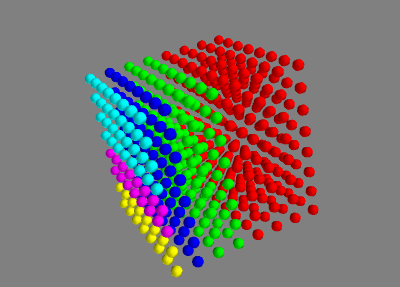
\includegraphics[height=1.2in]{figs/goodallocation}
        \caption{Contiguous}
        \label{fig:overview_sub1}
    \end{subfigure}%
    \hspace{1em}%
    \begin{subfigure}[t]{0.22\textwidth}
        \centering
        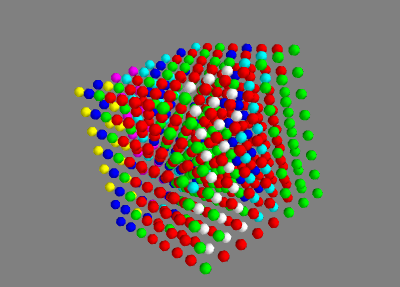
\includegraphics[height=1.2in]{figs/badallocation}
        \caption{Non-contiguous}
        \label{fig:overview_sub2}
    \end{subfigure}%
   \caption{Multiple jobs running concurrently with different allocations. 
   Each job is represented by a specific color. 
   a) shows the effect of contiguous job placement, 
   which could possibly reduce the inter-job interference. 
   b) shows non-contiguous job placement, 
   which may introduce both intra and inter-job interference. 
   }
   \label{fig:overview}
\end{figure}

When submitting jobs to HPC systems, 
users request system resources by specifying the number of compute nodes and expected runtime. 
The batch scheduler is then responsible for dispatching the submitted jobs to the system. 
Typically, there are multiple jobs running concurrently on the system,
resulting in the shared use of resources, particularly network links. 
A prominent problem with this network sharing is the contention over
the network among those concurrently running jobs. 
The network contention can cause communication variability and 
performance degradation to those jobs~\cite{abhinav-sc13}. 
This performance degradation can propagate into the queueing time of the following submitted jobs, 
thus leading to low system throughput and utilization~\cite{jose-ipdps15}. 
This adverse effect of network sharing can be mitigated by 
providing jobs with isolated allocations and exclusive network resources.

On the widely used torus-connected HPC systems~\cite{bgq,tofu,titan}, 
two job placement policies are commonly used. 
In \emph{contiguous placement} policy, 
each job gets a compact and contiguous set of computing nodes, 
as shown in Figure~\ref{fig:overview_sub1}. 
The partition-based placement adopted on the Blue Gene 
series systems is an example of contiguous placement policy~\cite{bgloverview}. 
The contiguous placement favors application performance 
through exclusive networking within a compact partition 
and the locality that implies. 
However, contiguous placement can cause both internal fragmentation 
(when more nodes are allocated to a job than it requests) 
and external fragmentation 
(when sufficient nodes are available for a request, but they can not be allocated contiguously), 
therefore leading to lower system utilization than is otherwise possible. 
On the other hand, the \emph{non-contiguous placement} policy, 
adopted by the Cray XT/XE series~\cite{carl-cug}, 
assigns free nodes to jobs regardless of contiguity, 
though of course efforts are made to maximize locality. 
Figure~\ref{fig:overview_sub2} shows the effect of non-contiguous placement. 
While eliminating internal and external fragmentation as seen in contiguous placement systems, 
in return non-contiguous placement policy introduces contention between jobs due to the interleaving of job nodes. 
The non-contiguous job placement can significantly reduce job performance, 
especially for communication-intensive ones~\cite{abhinav-sc13}.

We envision that future HPC systems will be equipped with 
a flexible job placement mechanism which combines the 
best of both contiguous and non-contiguous policy. 
Such a flexible job placement mechanism should take 
shared resource needs (e.g., network resources) of jobs into account 
when making scheduling and allocation decisions. 
With the knowledge and analysis of job communication patterns, 
it can be identified which jobs require exclusive network and compact allocation, and to what degree. 
Then, rather than allocating each job in a ``know-nothing'' manner, 
one may specialize job placement policy so that, for example, 
only the jobs with stringent network needs are given compact, isolated allocations, 
resulting in maximized utilization and minimized perceivable resource contention effects.

In this work, we focus on an in-depth analysis of intra- and inter-job 
communication interference with different job placements on torus-connected HPC systems. 
Torus-based networks are used on six of the top 10 supercomputers 
on the June 2015 Top500 lists~\cite{top500}. 
The current generation of IBM Blue Gene/Q (BG/Q) supercomputers, 
such as Mira at Argonne Nation Laboratory and 
Sequoia at Lawrence Livermore National Laboratory, 
have their compute nodes connected by a 5D torus network~\cite{bgq}. 
The K computer from Japan uses the ``Tofu'' interconnected system, 
which has a 6D mesh/torus topology~\cite{tofu}. 
Titan, a Cray XK7 supercomputer located at the Oak Ridge Leadership Computing Facility (OLCF), 
has nodes connected in a 3D torus within the compute partition~\cite{titan}. 
Although our analyses are based on torus networks, 
the ideas conveyed in this work is applicable to networks with different topologies. 

We selected three signature applications from 
the DOE Design Forward Project~\cite{designforwardwebpage} as examples 
to conduct detailed study about the communication pattern of parallel applications. 
We use a sophisticated simulation toolkit named CODES 
(standing for Co-Design of Multi-layer Exascale Storage Architectures)~\cite{Jason-2011} 
as a research vehicle to evaluate the performance of these applications 
with various allocations in a controlled environment. 
We then analyze the intra- and inter-job interference 
by simulating these applications running concurrently with different allocations. 
We believe the insights presented in this work can be very useful 
for the design of future HPC batch schedulers and resource managers.


The rest of this paper is organized as follows. 
Section~\ref{sec:application study} describes the three representative applications 
from the DOE Design Forward Project for our study. 
Section~\ref{sec:codes} talks about the use of CODES as research vehicle for our work. 
%Section~\ref{sec:config study} shows the performance analysis of three applications on different torus networks. 
Section~\ref{sec:interference} provides detailed analysis about the intra- and inter-job interference 
among three applications on torus network with different allocations. 
Section~\ref{sec:discussion} introduces a path toward communication-pattern aware allocation strategies, 
given the results of our analysis. 
Section~\ref{sec:related_work} discusses related work. 
Finally, the conclusion is presented in Section~\ref{sec:conclusion}.






\section{Application Study}
\label{sec:application study}

%A parallel application usually conforms to a combination of several basic communication patterns\cite{roth}. At its different execution phases, the application's communication behavior may follow different basic patterns respectively. \textcolor{blue}{When we look into the data flow during application execution, most parallel applications start with broadcast operation to distribute the data from root process to other processes\textcolor{red}{ref needed here}, followed by a series of computation and communication that conforms to certain pattern, which is usually the dominant part of application's execution. Before the application come to completion, all the working process will return their results to the root directly or hierarchically.} Parallel application's communication pattern usually involves lots of factors, such as communication intensity, operation-to-operation dependencies and the ``critical path" in its communication topology graph, etc. In this work, we focus on the locality of application's rank-to-rank communication topology graph.

A parallel application usually conforms to a combination of several basic communication patterns~\cite{roth}. 
At its different execution phases, 
the application's communication behavior may follow certain basic patterns respectively. 
There are many profiling tools available to capture 
information regarding communication patterns of parallel applications~\cite{tau,mpip,sst,oxbow}. 
They can provide information such as the percentage of different MPI operations, 
communication topology, the amount of data transferred between processes, etc.

There are many applications running on HPC systems such as Mira~\cite{bgq} and Titan~\cite{titan}. 
These applications are communication intensive and conform to various communication patterns. 
In this work, we select three representative applications from the DOE Design Forward Project. 
Each application exhibits a distinctive communication pattern that is commonly seen in HPC applications. 
We believe that the communication patterns of these applications 
are representative of a wide array of applications running on leadership-class machines. 
Specifically, we study the Algebraic MultiGrid Solver (AMG), 
Geometric MultiGrid (MultiGrid) and CrystalRouter MiniApps. 
The communication matrix presented in Figure~\ref{fig:apps_communication_matrix}
are generated with the IPM~\cite{ipm} data gathered from publicly available traces~\cite{designforwardwebpage}.


\begin{figure*}[htp]
    \centering
    \begin{subfigure}[t]{0.32\textwidth}
        \centering
        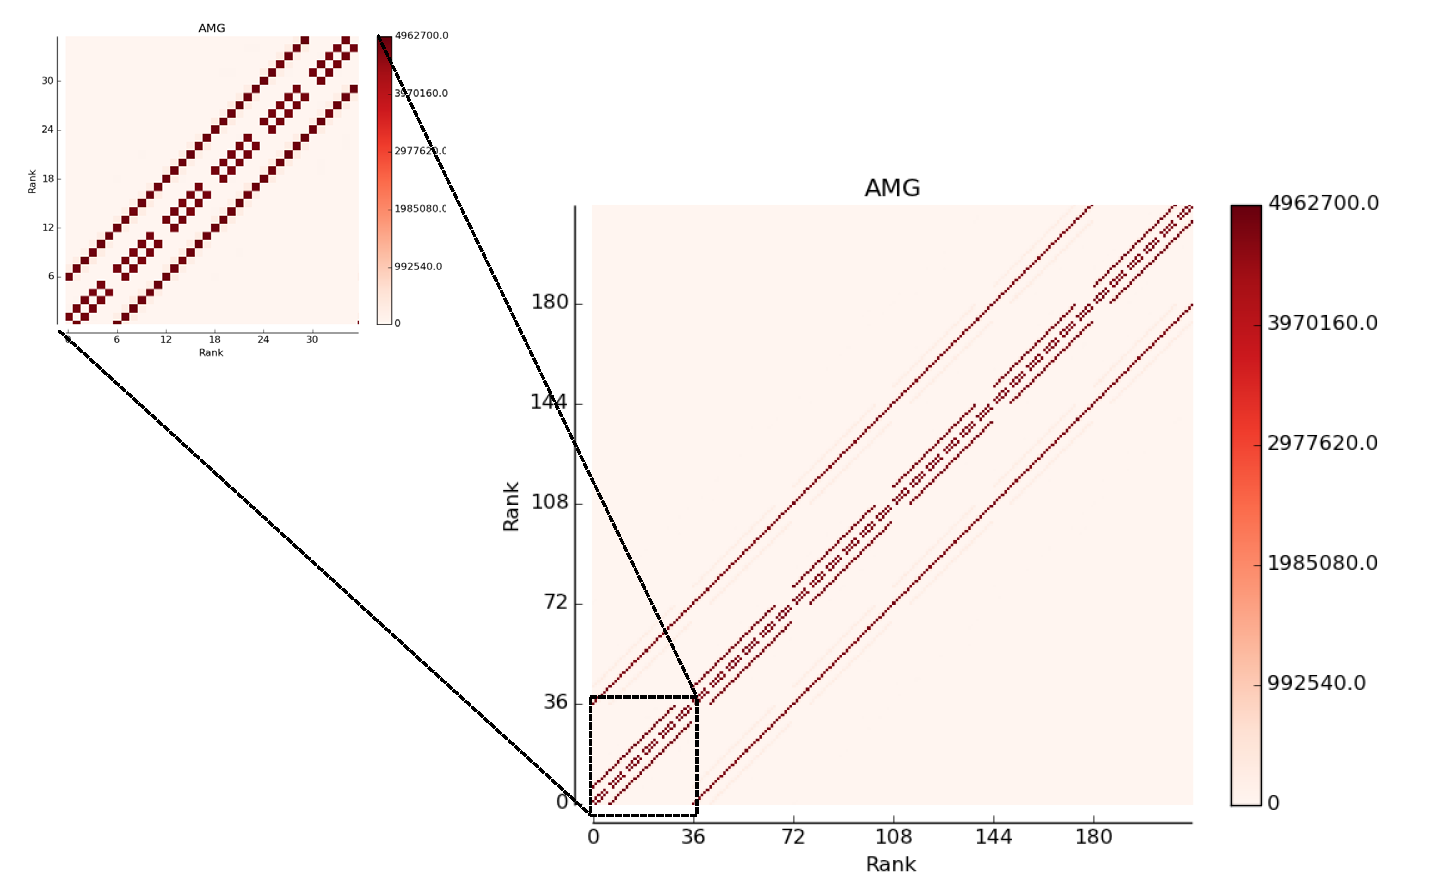
\includegraphics[height=1.5in]{figs/appstudy/amg/amg_pip}
        \caption{AMG}
        \label{fig:amg-communication-topology}
    \end{subfigure}
    \begin{subfigure}[t]{0.32\textwidth}
        \centering
        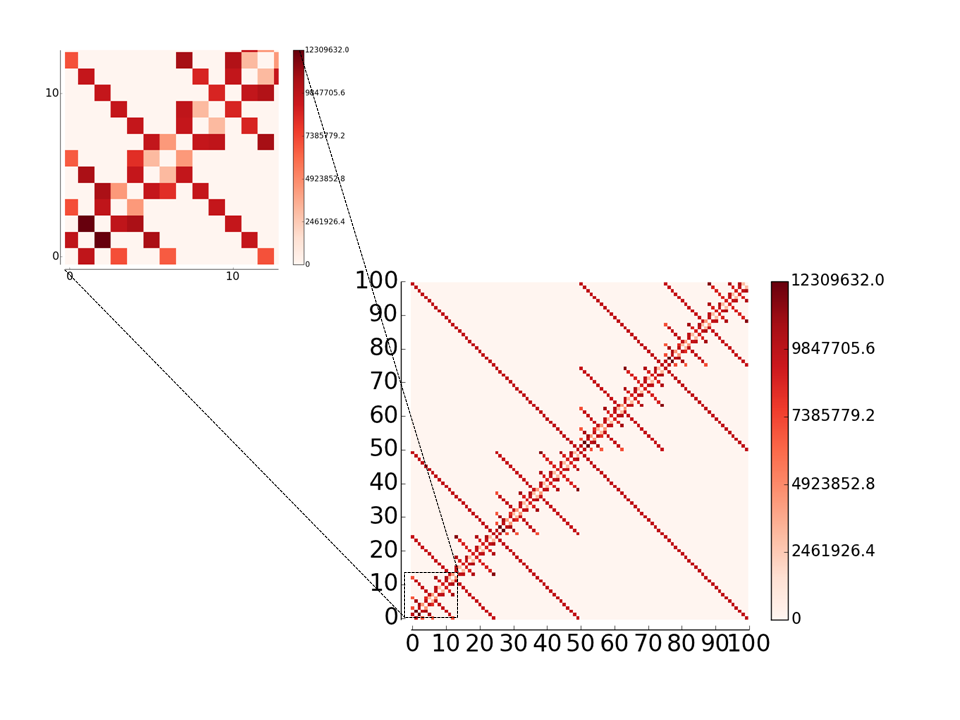
\includegraphics[height=1.5in]{figs/appstudy/cr/cr_pip}
        \caption{CrystalRouter}
        \label{fig:cr-communication-topology}
    \end{subfigure}
    \begin{subfigure}[t]{0.32\textwidth}
        \centering
        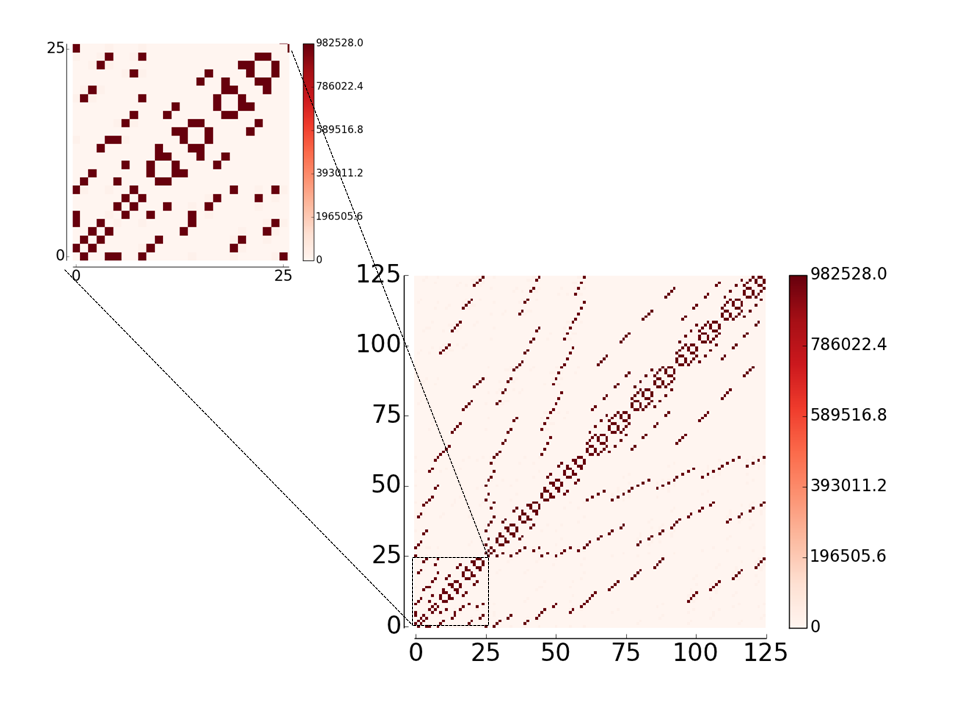
\includegraphics[height=1.5in]{figs/appstudy/mg/mg_pip}
        \caption{MultiGrid}
        \label{fig:mg-communication-topology}
    \end{subfigure}
    \caption{Applications rank-to-rank communication topology graph.}
    \label{fig:apps_communication_matrix}
\end{figure*}


\subsection{AMG}
\label{sec:amg}

%\begin{figure}[t!]
%    \centering
%    \begin{subfigure}[t]{0.25\textwidth}
%        \centering
%        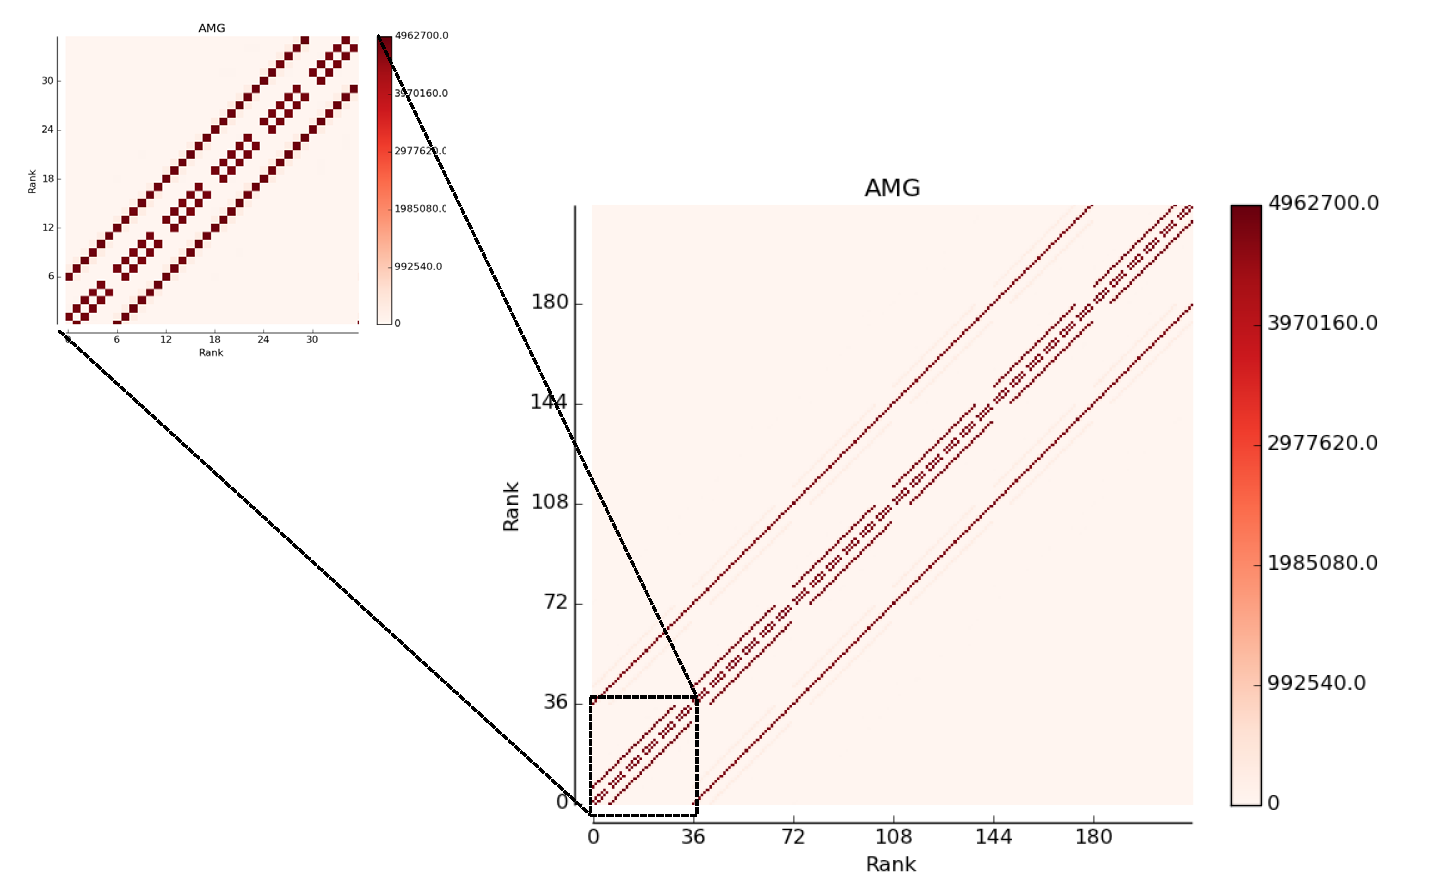
\includegraphics[height=1.5in]{figs/appstudy/amg/amg_pip}
%        \caption{}
%        \label{fig:amg-communication-topology}
%    \end{subfigure}%
%    ~
%    \begin{subfigure}[t]{0.24\textwidth}
%        \centering
%        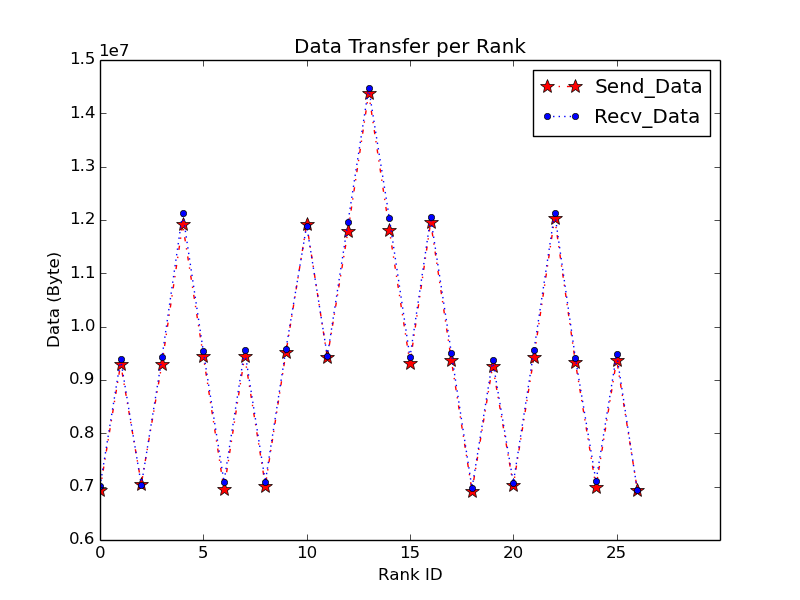
\includegraphics[height=1.2in]{figs/appstudy/amg/amg_data_transfer}
%        \caption{}
%        \label{fig:amg-data-trans}
%    \end{subfigure}
%    \caption{AMG. (a) Rank-to-rank communication topology graph, shows the intensity of communication between ranks in AMG. (b) The amount of data sent/received by each rank in AMG. Y-axis labels the amount of data transferred in MB, x-axis labels 216 ranks of AMG. }
%\end{figure}

The Algebraic MultiGrid Solver, or AMG, 
is a parallel algebraic multi-grid solver for linear systems arising from problems on unstructured mesh physics packages. 
It has been derived directly from the BoomerAMG solver 
that is being developed in the Center for Applied Scientific Computing (CASC) at LLNL \cite{amg}. 
The dominant communication pattern is regional communication 
with decreasing message size for different parts of the multi-grid v-cycle.

Figure~\ref{fig:amg-communication-topology} shows the communication matrix 
of a small scale AMG execution with 216 MPI Ranks. 
Note that the dominant communication pattern of the application doesn't change with scale. 
We can make the observation that AMG's dominant communication pattern is 3D Nearest Neighbor, 
each rank has intensive communication with up to six neighbors, 
depending on the boundaries of the ranks. 
Applications with similar pattern include PARTISN~\cite{partisn} and SNAP~\cite{snap}.


\subsection{Crystal Router}
\label{sec:crystalrouter}

%\begin{figure}[t!]
%    \centering
%    \begin{subfigure}[t]{0.25\textwidth}
%        \centering
%        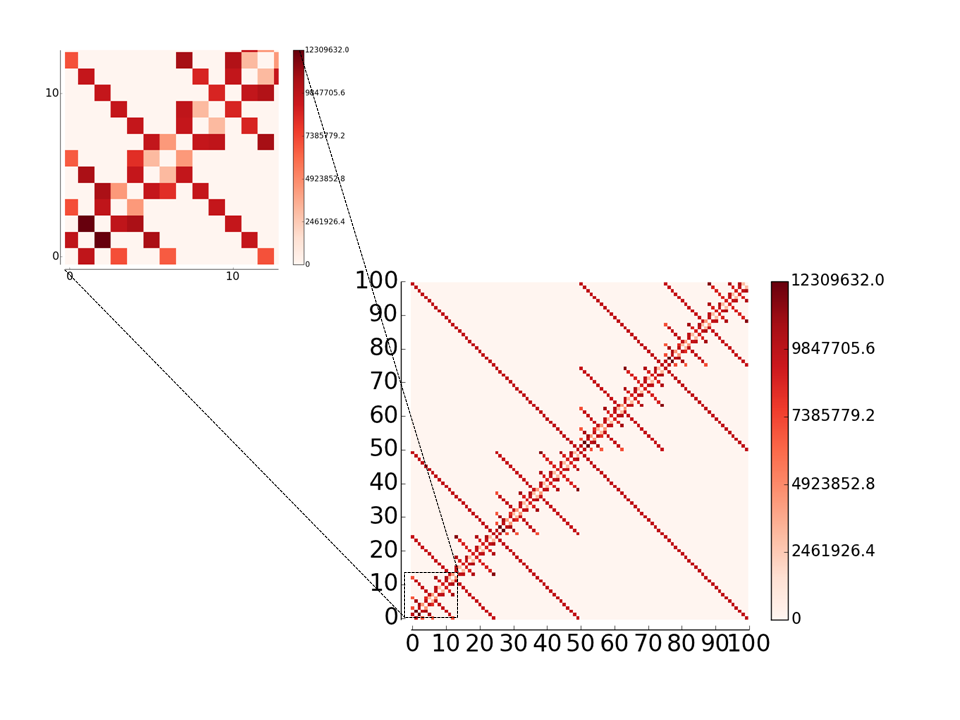
\includegraphics[height=1.5in]{figs/appstudy/cr/cr_pip}
%        \caption{Communication Topology}
%        \label{fig:cr-communication-topology}
%    \end{subfigure}
%    ~
%    \begin{subfigure}[t]{0.22\textwidth}
%        \centering
%        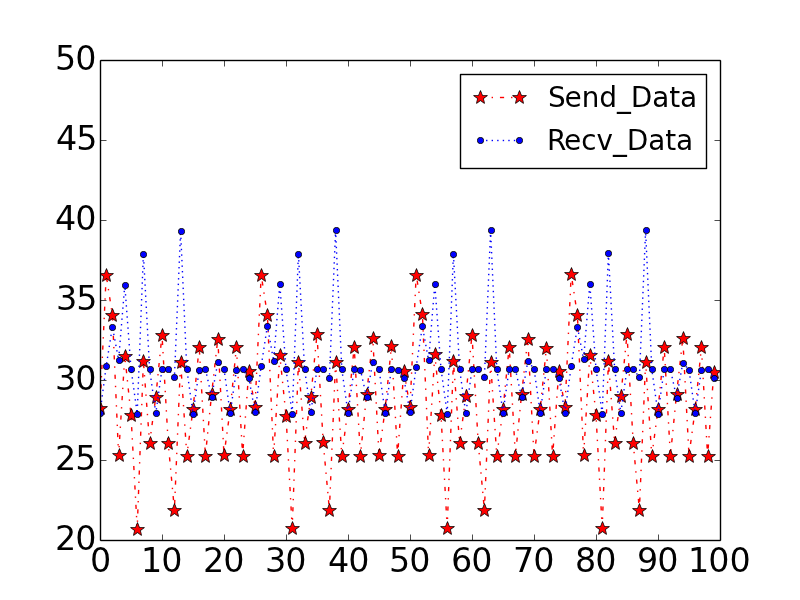
\includegraphics[height=1.2in]{figs/appstudy/cr/cr_data_transfer}
%        \caption{Data Volume}
%        \label{fig:cr-data-trans}
%    \end{subfigure}
%    \caption{CrystalRouter. (a) Rank-to-rank communication topology graph, shows the intensity of communication between ranks in CrystalRouter. (b) The amount of data sent/received by each rank in CrystalRouter. Y-axis labels the amount of data transferred in MB, x-axis labels 100 ranks of CrystalRouter. }
%\end{figure}

The second MiniApp covered is CrystalRouter, 
the extracted communication kernel of the full application Nek5000~\cite{nek5000}, 
which is a spectral element CFD application developed at Argonne National Laboratory. 
It features spectral element multi-grid solvers coupled with a highly scalable, 
parallel coarse-grid solver that is widely used for projects including ocean current modeling, 
thermal hydraulics of reactor cores, and spatiotemporal chaos. 
CrystalRouter demonstrates the ``many-to-many'' communication pattern 
through a scalable multi-stage communication process. 
The way CrystalRouter works is the nodes compute for a while, 
then synchronize and communicate, continually alternating between these two types of activities.

The collective communication in CrystalRouter utilizes a recursive doubling approach. 
Ranks in CrystalRouter conform to a $n$-dimensional hypercube 
and recursively split into ($n$-1)-dimensional hypercubes, 
with communication occurring along the splitting plane. 
The pattern of this communication can be found in Figure~\ref{fig:cr-communication-topology}. 
By nature of the logarithmic splitting process, 
a substantial portion of the communication occurs in small neighborhoods of ranks. 
CrystalRouter represents a group of applications whose dominant communication 
is a hybrid of multi-stage local and hierarchical global communication, 
and shares similarities with most MPI collective communication implementations.


\subsection{MultiGrid}
\label{sec:multigrid}

%\begin{figure}[t!]
%    \centering
%    \begin{subfigure}[t]{0.25\textwidth}
%        \centering
%        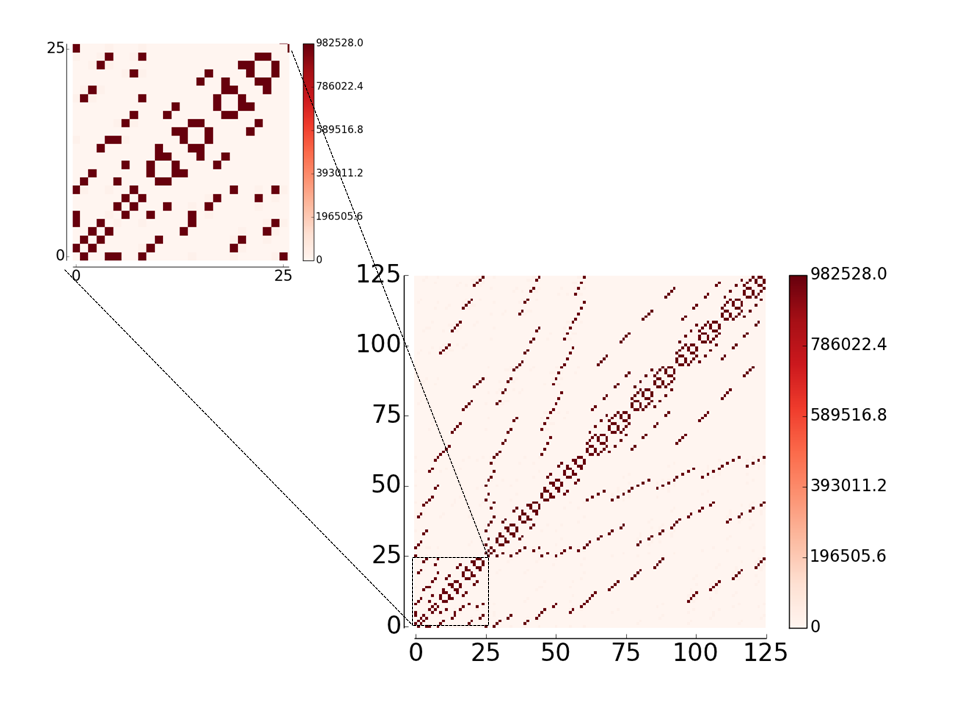
\includegraphics[height=1.5in]{figs/appstudy/mg/mg_pip}
%        \caption{Communication Topology}
%        \label{fig:mg-communication-topology}
%    \end{subfigure}
%    ~
%    \begin{subfigure}[t]{0.22\textwidth}
%        \centering
%        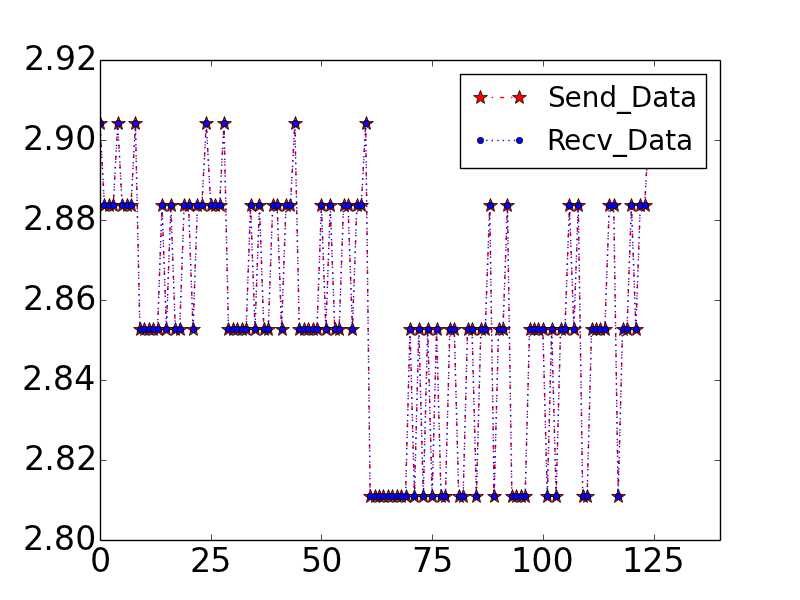
\includegraphics[height=1.2in]{figs/appstudy/mg/mg_data_transfer}
%        \caption{Data Volume}
%        \label{fig:mg-data-trans}
%    \end{subfigure}
%    \caption{MultiGrid. (a) Rank-to-rank communication topology graph, shows the intensity of communication between ranks in MultiGrid. (b) The amount of data sent/received by each rank in MultiGrid. Y-axis labels the amount of data transferred in MB, x-axis label 125 ranks of MultiGrid. }
%\end{figure}

MultiGrid is geometric multi-grid v-cycle from the production elliptic solver BoxLib, 
a software framework for massively parallel block-structured adaptive mesh refinement (AMR) codes~\cite{boxlib}. 
MultiGrid conforms to many-to-many communication pattern with decreasing message size and 
collectives for different parts of the multi-grid v-cycle. 
It is widely used for structured grid physics packages. 

Figure~\ref{fig:mg-communication-topology} shows the communication matrix of MultiGrid with 125 ranks. 
We can see intensive communication along the diagonal that resembles nearest neighbor communication, similar to AMG. 
However, the communication topology leads to a greater ``spread'' of communication across the set of ranks, 
challenging the maximization of communication locality with respect to ranks. 
In this sense, it can be considered a ``many-to-many'' pattern. 
Applications with such similar dominant communication pattern are like FillBoundary, another PDE solver code in~\cite{boxlib}.



\section{Research Vehicle}
\label{sec:codes}

It is difficult to accurately and flexibly experiment with concurrently running jobs in an HPC context. 
One reason is that the allocation strategy used on production machine is part of the system software, 
which can not be changed by users. 
Even the system administrator is not authorized to make that change. 
Another reason is that it is unrealistic to reserve the system exclusively 
to run the same job with desired allocation without interference and 
then compare the results with those in the presence of interference. 
Therefore, we resort to simulation for this work.


A simulation toolkit named CODES enables the exploration of simulating 
different HPC networks at flit-level with high fidelity~\cite{Jason-2011, mubarak-sc2012}. 
CODES is built on top of Rensselaer Optimistic Simulation System (ROSS) parallel discrete-event simulator~\cite{ross}, 
which is capable of processing billions of events per second on leadership-class supercomputers. 
CODES support both torus and dragonfly network with high fidelity flit-level simulation. 
CODES has this network workload component that is capable of conducting trace-driven simulations. 
It can take MPI application traces generated by SST DUMPI \cite{sst} to drive CODES network models. 
In this work, we focus on an in-depth analysis of intra- and inter-job 
communication interferences with different job allocations on torus-connected HPC systems. 
Torus networks have been extensively used in the current generation of supercomputers 
because of their linear scaling on per-node cost and competitive communication performance.



%\section{Configuration Study}
\label{sec:config study}

In this section, we study the communication behavior of three applications on torus networks with different dimensionality and bandwidth configurations. Torus networks are $k$-ary $n$-cubes, with $k^{n}$ nodes in total arranged in an $n$-dimensional grid having $k$ nodes in each dimension. Each node has $2\times n$ direct linked neighbor nodes with wraparound. In these and all following experiments, non-adaptive routing is used. While making specific recommendations as to an ``optimal'' network configuration for a given application is out of the scope of this study, the experiments do highlight the nuances inherent in design choices such as network diameter and bandwidth planning.

We perform three sets of experiments. Each looks at per-rank distribution of performance of AMG, CrystalRouter and MultiGrid on a set of 2048-node torus models, one with $n=3$ ($16^{2} \times 8$), one with $n=5$ ($8\times 4^{4}$), and one with $n=7$ ($4^{4} \times 2^{3}$). Performance in this context is defined by the total message transfer time for each sending rank, which we are able to precisely measure due to the simulation environment providing us with an absolute notion of time. Note that we simply perform linear rank assignment, one per node -- later sections investigate rank and node mapping effects. In the first, shown in Figure~\ref{fig:dimensionality-study}, we keep the link bandwidth constant at 2GiB/s in each direction, corresponding to Blue Gene/Q systems~\cite{bgq}, leading to aggregate node bandwidths of 12GiB/s, 20GiB/s, and 28GiB/s for the 3D, 5D, and 7D tori, respectively. In the second, shown in Figure~\ref{fig:bandwidth-study}, we fix the torus dimensionality to 5D. In the third, shown in Figure~\ref{fig: bandwidth-time-box}, we instead fix the per-node aggregate bandwidth (and thus the system aggregate bandwidth) and modify the torus dimensionality, resulting in per-link bandwidths shown in Table~\ref{tab: fix-bandwidth}.

\begin{figure*}[t!]
    \centering
    \begin{subfigure}[t]{0.32\textwidth}
        \centering
        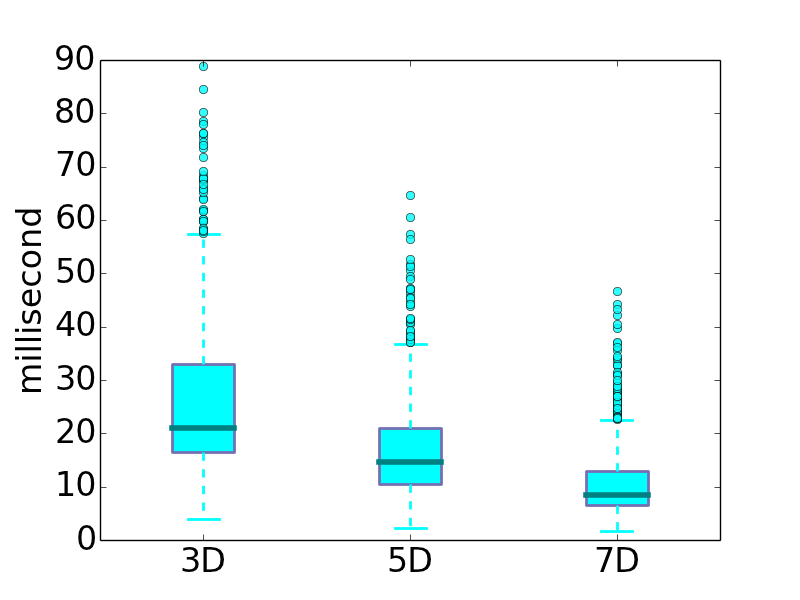
\includegraphics[height=1.5in]{figs/dimenstudy/amg_box}
        \caption{AMG}
        \label{fig:dimen-amg}
    \end{subfigure}%
    \hspace{1em}%
    \begin{subfigure}[t]{0.32\textwidth}
        \centering
        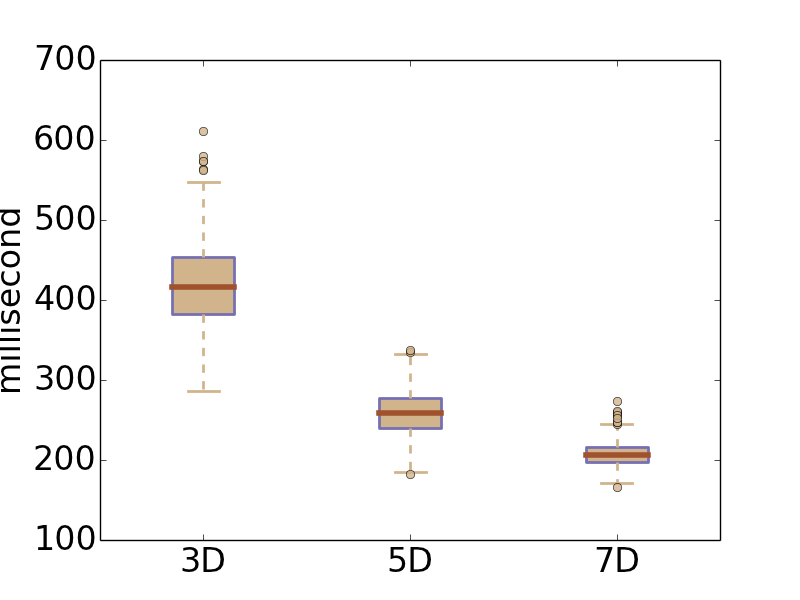
\includegraphics[height=1.5in]{figs/dimenstudy/cr_box}
        \caption{CrystalRouter}
        \label{fig:dimen-cr}
    \end{subfigure}%
    \begin{subfigure}[t]{0.32\textwidth}
        \centering
        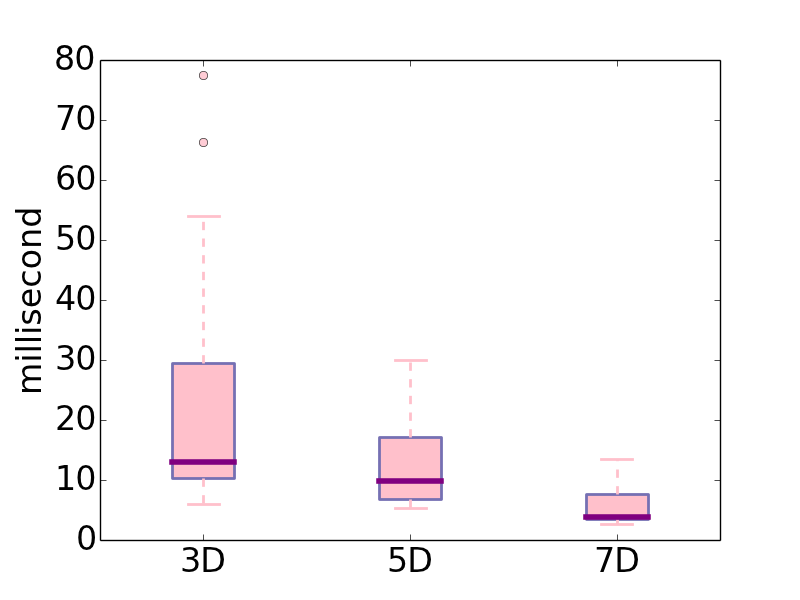
\includegraphics[height=1.5in]{figs/dimenstudy/mg_box}
        \caption{MultiGrid}
        \label{fig:dimen-mg}
    \end{subfigure}%
   \caption{Data Transfer Time of AMG, CrystalRouter and MultiGrid on 3D, 5D and 7D torus network, with constant per-link bandwidth.}
   \label{fig:dimensionality-study}
\end{figure*}

In the fixed link bandwidth experiment, shown in Figure~\ref{fig:dimensionality-study}, the data transfer time of the three applications are significantly reduced as the dimensionality increases, so the applications can easily make use of the increased dimensionality (lower hops on average) and/or aggregate bandwidth (more links being concurrently used). Interestingly, AMG has the greatest degree of outliers compared to the others. We expect this to be a combination of non-optimal rank mappings causing a greater degree of variance due to the highly regular communication pattern and the distribution of message sizes. MultiGrid seems to benefit the most in terms of reducing the spread of the time distribution, though the median message time remains roughly within a factor of two. The time distribution in CrystalRouter seems to accrue the most benefits, likely due to the combination of cross-cutting and localized per-rank traffic.

\begin{figure*}[t!]
    \centering
    \begin{subfigure}[t]{0.32\textwidth}
        \centering
        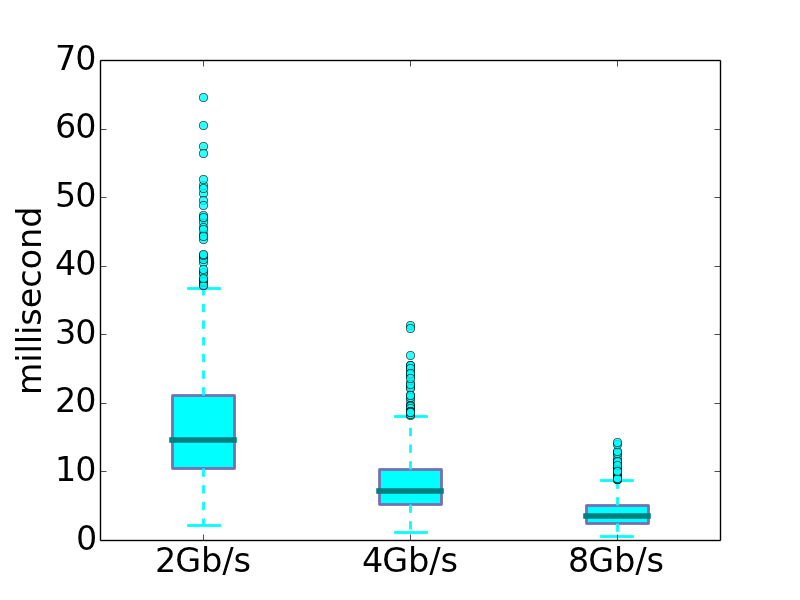
\includegraphics[height=1.5in]{figs/bandwidthstudy/amg_bw_box}
        \caption{AMG}
        \label{fig:bdwstudy-amg}
    \end{subfigure}%
    \hspace{1em}%
    \begin{subfigure}[t]{0.32\textwidth}
        \centering
        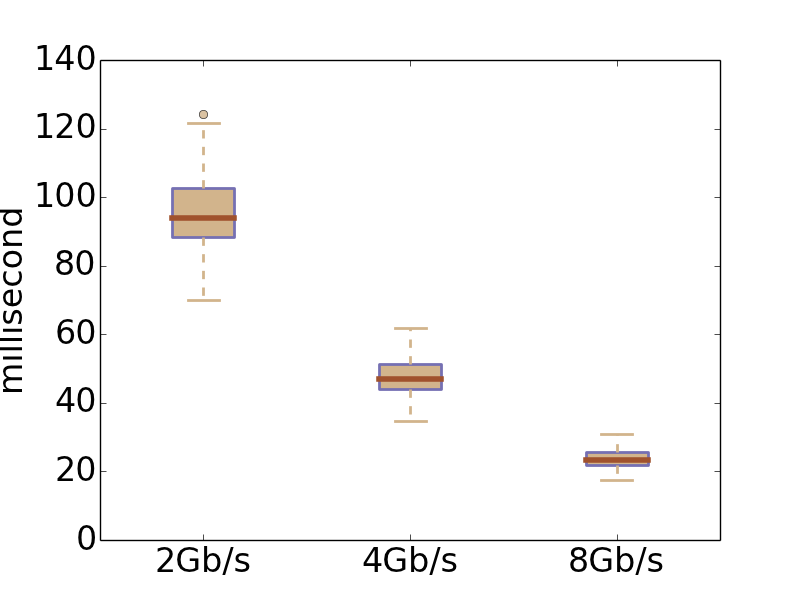
\includegraphics[height=1.5in]{figs/bandwidthstudy/cr_bw_box}
        \caption{CrystalRouter}
        \label{fig:bdwstudy-cr}
    \end{subfigure}%
    \begin{subfigure}[t]{0.32\textwidth}
        \centering
        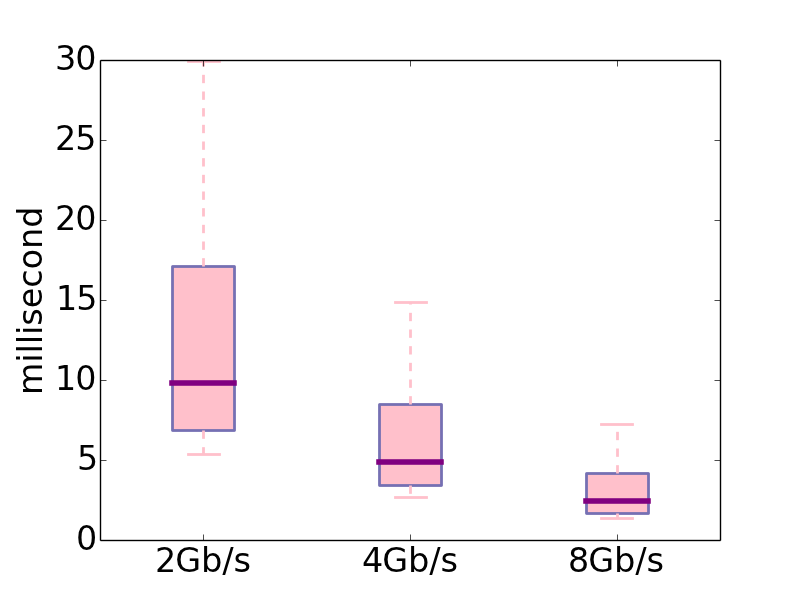
\includegraphics[height=1.5in]{figs/bandwidthstudy/mg_bw_box}
        \caption{MultiGrid}
        \label{fig:bdwstudy-mg}
    \end{subfigure}%
   \caption{Data transfer time of AMG, CrystalRouter and MultiGrid on 5D torus network with 2GiB/s, 4GiB/s and GiB/s direct link bandwidth. }
   \label{fig:bandwidth-study}
\end{figure*}

In the fixed dimensionality experiment, shown in Figure~\ref{fig:bandwidth-study}, the increased per-link bandwidth, expectedly, benefits each application roughly equally, reducing the time distributions linearly.

\begin{figure*}[t!]
    \centering
    \begin{subfigure}[t]{0.32\textwidth}
        \centering
        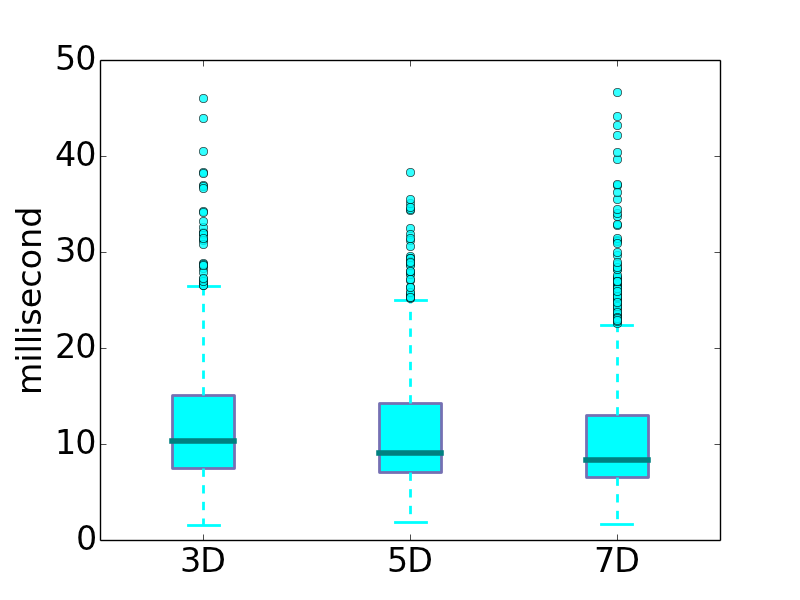
\includegraphics[height=1.5in]{figs/samebdw/amg}
        \caption{AMG}
        \label{fig:samebd-amg}
    \end{subfigure}%
    \hspace{1em}%
    \begin{subfigure}[t]{0.32\textwidth}
        \centering
        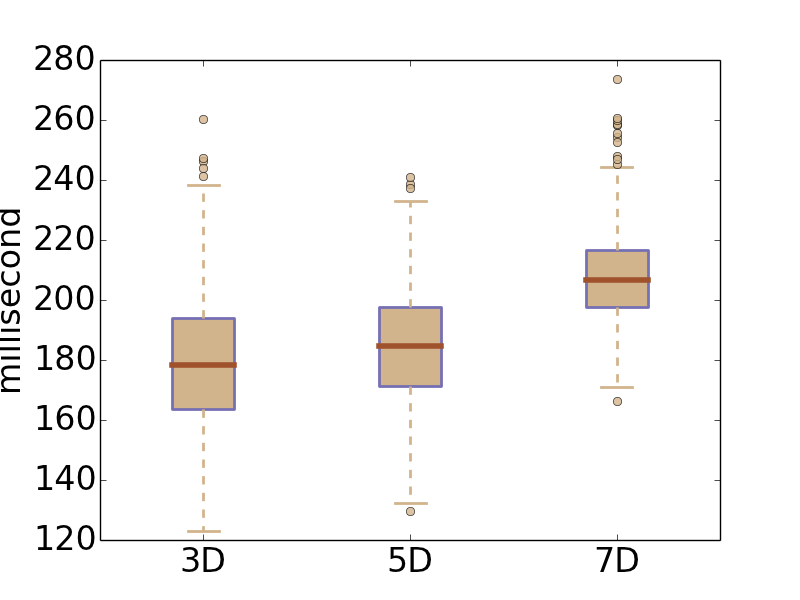
\includegraphics[height=1.5in]{figs/samebdw/cr}
        \caption{CrystalRouter}
        \label{fig:samebd-cr}
    \end{subfigure}%
    \begin{subfigure}[t]{0.32\textwidth}
        \centering
        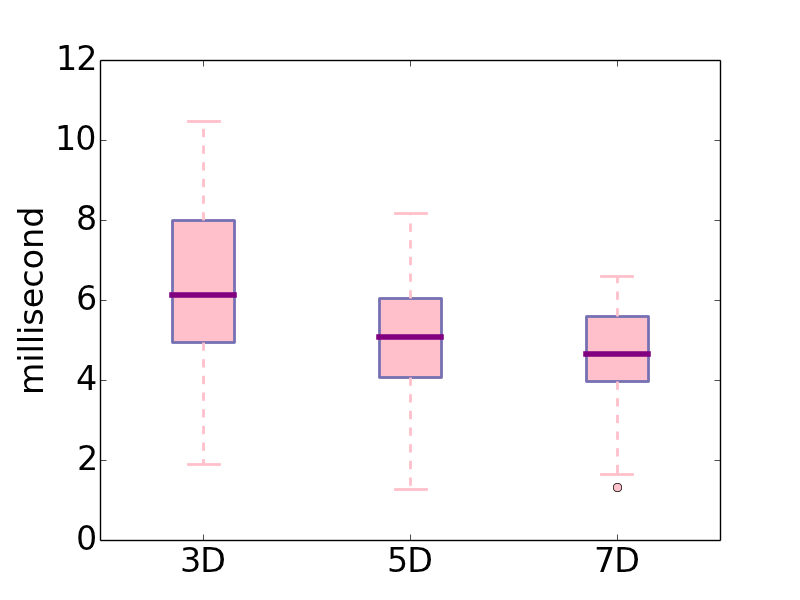
\includegraphics[height=1.5in]{figs/samebdw/mg}
        \caption{MultiGrid}
        \label{fig:samebd-mg}
    \end{subfigure}%
   \caption{Data transfer time of AMG, CrystalRouter and MultiGrid on 3D, 5D and 7D torus network with same aggregated bandwidth. }
   \label{fig: bandwidth-time-box}
\end{figure*}

\begin{table}[ht]
\begin{center}
\caption{Torus networks with same aggregated bandwidth} 
\label{tab: fix-bandwidth}
\begin{tabular}{l c c c} 
\toprule % Top horizontal line
\toprule
&\multicolumn{3}{c}{Bandwidth } \\
\cmidrule(l){2-4}
Dimension  & per-link & aggregate &\\ % Column names row
\midrule % In-table horizontal line
3D      & 4.67GiB/s  & 28GiB/s  & \\  % Content row 1
\midrule % In-table horizontal line
5D    & 2.8GiB/s  & 28GiB/s  &\\ % Content row 1
\midrule % In-table horizontal line
7D    & 2GiB/s & 28GiB/s & \\
\midrule
\bottomrule % Bottom horizontal line
\end{tabular}
\end{center}
\end{table}

In the fixed aggregate bandwidth experiment, with configuration in Table~\ref{tab: fix-bandwidth} and results shown in Figure~\ref{fig: bandwidth-time-box}, the results are more nuanced. At least for these applications, the benefits from increased dimensionality do not outweigh the reduction in per-link bandwidth. MultiGrid does see benefits in the increased dimensionality, particularly with respect to outliers, but has a similar median message time. CrystalRouter reduces performance as the dimensionality increases, but only by a small degree. AMG remains roughly the same, minus a dip in the maximum message time that could be due to rank-to-node mapping changes.




\section{Interference Analysis}
\label{sec:interference}

\textbf{\emph{Intra-job interference}} refers to the network 
contention between ranks within each application. 
\textbf{\emph{Inter-job interference}} is introduced by concurrently 
running jobs that adjacent to each other sharing network resources. 
Communication variability due to such interference can 
cause application performance degradation.

In this section we will study both kinds of interference 
in the context of a torus network. 
Since application's communication pattern won't change with its scale, 
we use AMG with 216 ranks, CrystalRouter with 100 ranks, and MultiGrid 125 ranks. 
And in order to accommodate three applications running concurrently with different allocations, 
we simulate a 2K-node 3D torus ($16^{2} \times 8$) network for the experiments.


\subsection{Intra-Job Interference Analysis}
\label{sec: introjob}

We design two sets of experiments to study the 
intra-job interference of each application. 
In the first, shown in Figure \ref{fig:shapestudy}, 
we assign each application with allocations in \emph{three different shapes}. 
In the second, shown in Figure \ref{fig:diffmap}, 
we study the intra-job interference by using different 
mapping strategies for each application with given allocation shape. 

In the allocation shapes experiment, 
we select three possible shapes commonly seen on the 3D torus network. 
They are 3D balanced-cube, 3D unbalanced-cube and 2D mesh, 
as shown in Figure \ref{fig:alloc-shapes}.

3D balanced-cube, shown as red in Figure \ref{fig:cont_sub1}, 
can guarantee the minimum \emph{average pair-wise distance} within the allocation. 
Some research studies~\cite{leung,abhinav-sc13} indicate that 
compact allocation can guarantee jobs with better performance. 
They use a variety of metrics to evaluate the compactness of the allocation, 
such as \emph{average pair-wise distance}, \emph{diameter} and \emph{contiguity}. 
In this work, we select 3D balanced-cube as the most compact allocation on a 3D torus network.

3D unbalanced-cube, shown in green color in Figure \ref{fig:cont_sub1}, 
is a rectangular prism, which is the possible allocation shape 
on the systems with asymmetric networks. 
For example, Cray XE6/XK7 systems are deployed 3D tori with Gemini routers. 
The network connections in the \emph{y}-direction have 
only half the bandwidth of the cables used in the \emph{x} and \emph{z} directions. 
In order to take advantage of the faster links in the \emph{x} and \emph{z} directions, 
job allocation starts from X-Z plane, 
which leads to a rectangular prism shaped allocation~\cite{RF}.

2D mesh, shown as blue in Figure \ref{fig:cont_sub1}, 
can be cut out from a single layer of the 3D torus. 
2D mesh is a very common allocation shape on the torus network 
for both contiguous and non-contiguous placement policies. 
For example, Cray Application Level Placement Scheduler (ALPS) indexes 
all compute nodes in a torus network into a list and 
makes job allocation by simply going through that list~\cite{carl-cug}. 
When the list is obtained by sorting the nodes based on 
their spacial coordinates in the torus, 
allocation made off from this list will be 2D mesh. 
The IBM Blue/Gene Q supercomputer Mira at Argonne Leadership Computing Facility 
also allow its allocation partition configured into mesh~\cite{zhou-ipdps}. 

\begin{figure*}[t!]
    \centering
    \begin{subfigure}[t]{0.22\textwidth}
        \centering
        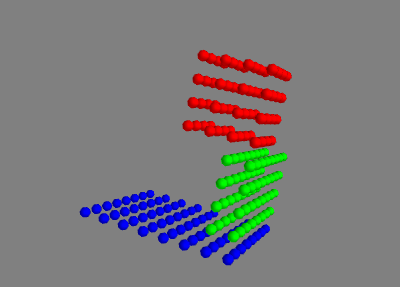
\includegraphics[height=1.2in]{figs/allocshape/allocation}
        \caption{ }
        \label{fig:cont_sub1}
    \end{subfigure}%
    \hspace{1em}%
    \begin{subfigure}[t]{0.22\textwidth}
        \centering
        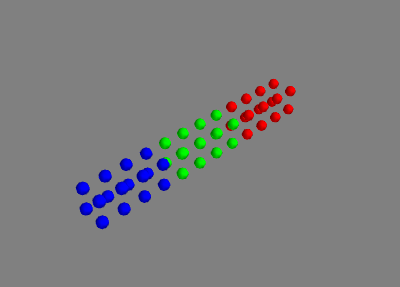
\includegraphics[height=1.2in]{figs/allocshape/unitsize/unit16}
        \caption{ }
        \label{fig:noncont_sub1}
    \end{subfigure}%
    \hspace{1em}%
    \begin{subfigure}[t]{0.22\textwidth}
        \centering
        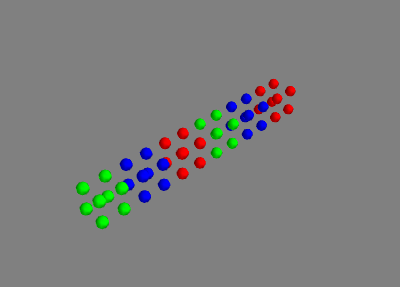
\includegraphics[height=1.2in]{figs/allocshape/unitsize/unit8}
        \caption{ }
        \label{fig:noncont_sub2}
    \end{subfigure}%
    \hspace{1em}%
    \begin{subfigure}[t]{0.22\textwidth}
        \centering
        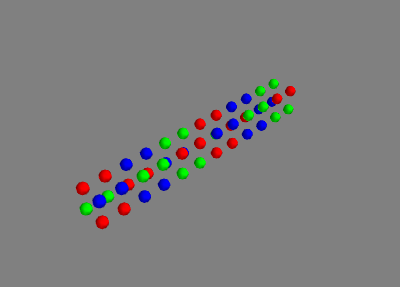
\includegraphics[height=1.2in]{figs/allocshape/unitsize/unit2}
        \caption{ }
        \label{fig:noncont_sub3}
    \end{subfigure}%
    \caption{
    (a) Contiguous allocation in three different shapes. 
    ``Blue" is a 2D mesh, ``Green" is a 3D-unbalanced cube and ``Red" is a 3D-balanced cube. 
    (b)-(d) Non-contiguous allocation. Each job is represented by a specific color. 
    The nodes assigned to different jobs are interleaved, 
    the size of allocation unit are 16, 8 and 2.
    }
    \label{fig:alloc-shapes}
\end{figure*}


AMG with 3D ``Nearest Neighbor" communication pattern takes less time 
when being assigned with 3D-unbalanced allocation than 3D-balanced, 
as shown in Figure~\ref{fig:shapstudy-amg}. 
And MultiGrid gets the best performance (shortest data transfer time) 
when running on 3D-balanced allocation, as shown in Figure~\ref{fig:shapstudy-mg}. 
Since MultiGrid's communication pattern is ``Many-to-Many" dominant, 
3D-balanced is the most compact allocation with shortest pair-wise distance between nodes, 
which can reduce the aggregated hops for transferring message among ranks in MultiGrid. 
Since CrystalRouter has both dominant local communication and multi-stage global data transfer, 
the 3D-balance is also the best allocation, but its advantage over 3D-unbalanced is not 
that obvious as to MultiGrid, as shown in Figure~\ref{fig:shapstudy-cr}.

Lots of research studies have designed complex placement algorithms 
to provide application with the most compact allocation~\cite{leung,LO}. 
However, as shown in our experiments, providing cubic allocation without 
considering application's communication pattern can not guarantee 
the best performance for every application. 
Compact allocation should be provided to applications with intensive global data transfer, 
such as those conforms to ``Many-to-Many" communication pattern. 
Applications with dominant communication pattern like ``Nearest Neighbor" 
can not fully utilize the compact allocation and 
may get even better performance on a relaxed allocation shape. 



\begin{figure*}[t!]
    \centering
    \begin{subfigure}[t]{0.32\textwidth}
        \centering
        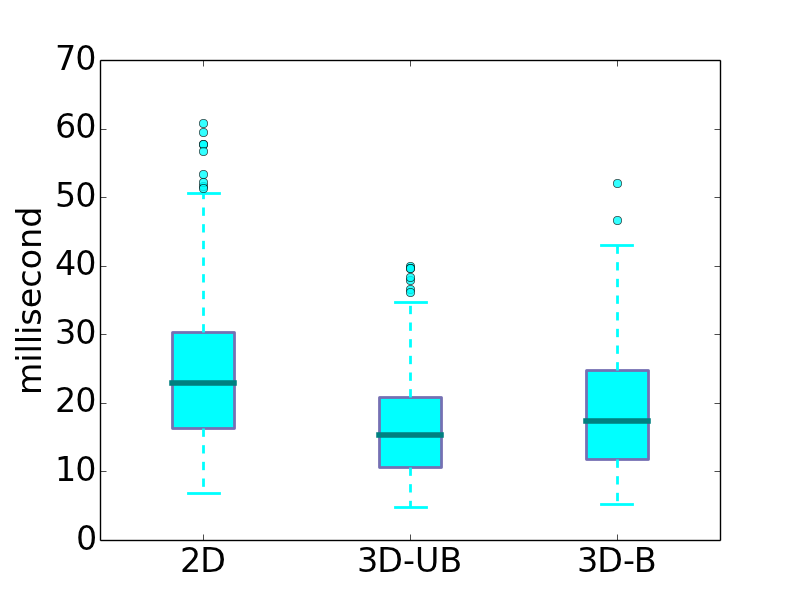
\includegraphics[height=1.5in]{figs/intra-job/shapestudy/amg_box}
        \caption{AMG}
        \label{fig:shapstudy-amg}
    \end{subfigure}%
    \hspace{1em}%
    \begin{subfigure}[t]{0.32\textwidth}
        \centering
        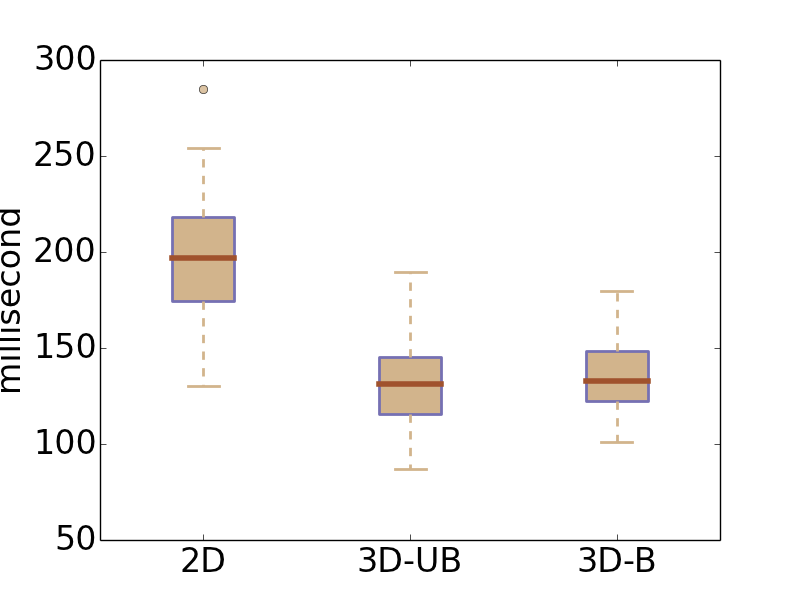
\includegraphics[height=1.5in]{figs/intra-job/shapestudy/cr_box}
        \caption{CrystalRouter}
        \label{fig:shapstudy-cr}
    \end{subfigure}%
    \begin{subfigure}[t]{0.32\textwidth}
        \centering
        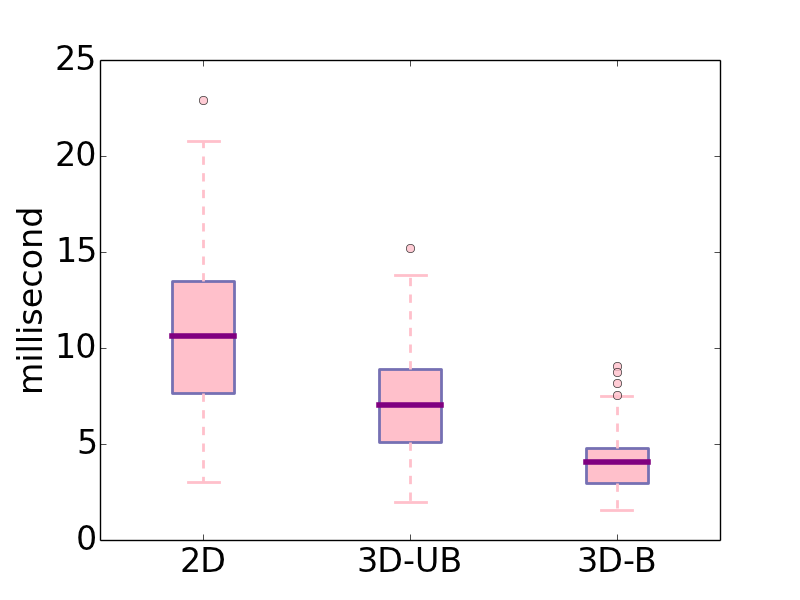
\includegraphics[height=1.5in]{figs/intra-job/shapestudy/mg_box}
        \caption{MultiGrid}
        \label{fig:shapstudy-mg}
    \end{subfigure}%
   \caption{
   Data transfer time of AMG, CrystalRouter and MultiGrid on 3D-balanced, 
   3D-unbalanced and 2D allocation.
   }
   \label{fig:shapestudy}
\end{figure*}


The rank-to-node mapping of parallel applications on HPC systems 
could greatly impact applications' performance. 
However, finding the optimal mapping solution for a given 
application is out the scope of this work. 
Our experiments aims to show how mapping strategies impact the 
intra-job interference of application with specific communication pattern.

We provide AMG, CrystalRouter and MultiGrid with 3D-balance allocation and 
use three mapping strategies to do the rank-to-node mapping. 
The ``Linear" mapping, as we used in the previous experiments, 
is to map each rank according to the dimensional ordering of compute nodes. 
The ``Cube" mapping assigns ranks into consecutive $2^{3}$ cubes. 
The ``Random" mapping assigns ranks randomly within the allocation. 

AMG remains roughly the same when it been mapped by ``Linear" and ``Cube", 
shown in Figure~\ref{fig:diffmap-amg}. 
Although ``Linear" and ``Cube" mapping strategies cause some routing overlap for AMG's communication, 
both mapping strategies still preserve the locality of AMG's ``3D Nearest Neighbor" communication pattern. 
The ``Random" mapping totally destroys AMG's communication pattern, 
and results in intra-job interference among all the ranks in AMG. 
The performance degradation caused by using ``Random" mapping is up to 90\%.

The ``Cube" mapping improves CrystalRouter's performance over the ``Linear" 
by reducing the pair-wise distance between ranks, shown in Figure~\ref{fig:diffmap-cr}. 
The global data transfer in CrystalRouter will takes fewer hops with ``Cube" mapping. 
The ``Random" mapping scatters the ranks within the local neighborhood 
of CrystalRouter and make their communication less efficient. 


The ``Cube" mapping benefits MultiGrid's ``Many-to-Many" communication. 
However, due to the small amount of data transfer among ranks in MultiGrid, 
``Cube" mapping fails to exhibit a drastic advantage. 
``Random" mapping neither cause too much degradation for the same reason, 
shown in Figure~\ref{fig:diffmap-mg}.


\begin{figure*}[t!]
    \centering
    \begin{subfigure}[t]{0.32\textwidth}
        \centering
        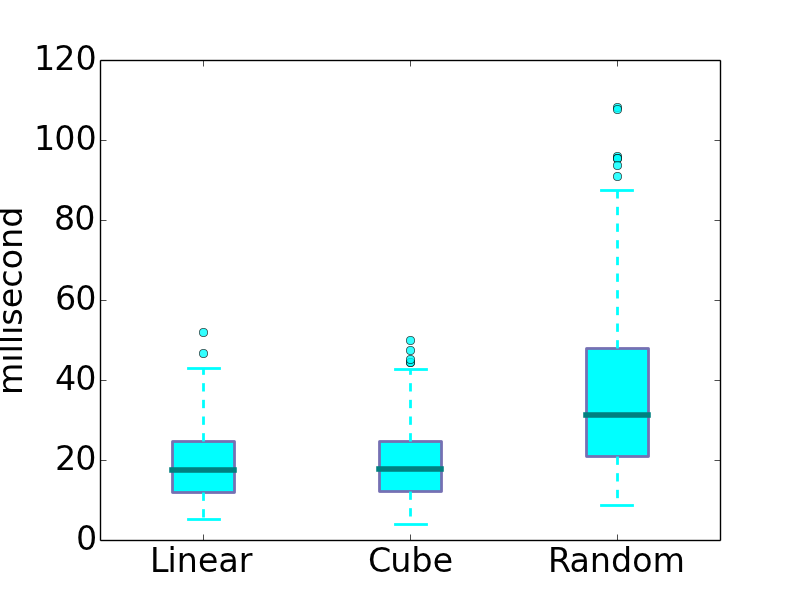
\includegraphics[height=1.5in]{figs/diffmapping/amg}
        \caption{AMG}
        \label{fig:diffmap-amg}
    \end{subfigure}%
    \hspace{1em}%
    \begin{subfigure}[t]{0.32\textwidth}
        \centering
        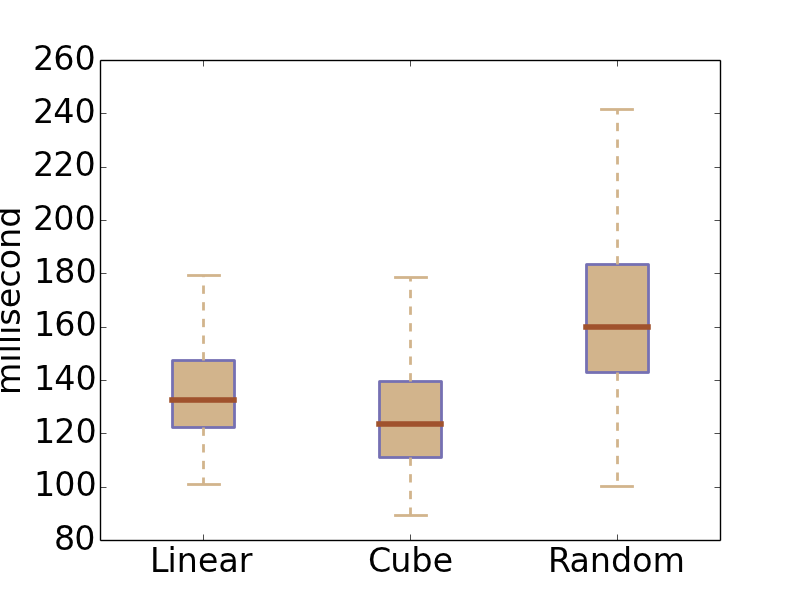
\includegraphics[height=1.5in]{figs/diffmapping/cr}
        \caption{CrystalRouter}
        \label{fig:diffmap-cr}
    \end{subfigure}%
    \begin{subfigure}[t]{0.32\textwidth}
        \centering
        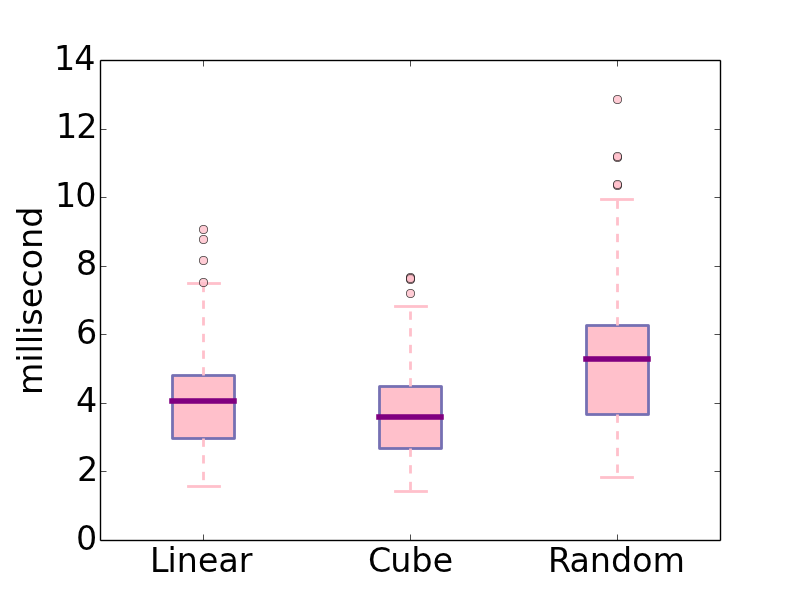
\includegraphics[height=1.5in]{figs/diffmapping/mg}
        \caption{MultiGrid}
        \label{fig:diffmap-mg}
    \end{subfigure}%
   \caption{
   Data transfer time of AMG, CrystalRouter and MultiGrid 
   on 3D-balanced allocation using  different mapping strategies.
   }
   \label{fig:diffmap}
\end{figure*}




\subsection{Inter-Job Interference Analysis}
\label{sec: interjob interference study}

Inter-job interference has been identified as one of the major culprits 
for application's performance variability~\cite{abhinav-sc13,skinner,rosenthal}. 
Inter-job interference is a more prominent issue for system adopted 
non-contiguous placement policy than systems with contiguous policy. 
Applications communication time have been demonstrated to 
vary from 36\% faster to 69\% slower due to job interference 
when they are running concurrently with non-contiguous allocations~\cite{abhinav-sc13}.

We assign each application with non-contiguous allocation and 
run them concurrently on the same network. 
The allocation unit belongs to different jobs are interleaved. 
In order to study the impact of different allocation unit size on 
applications' inter-job interference, 
we conduct experiments with unit size of 16, 8 and 2, 
shown respectively in Figure~\ref{fig:noncont_sub1}, 
~\ref{fig:noncont_sub1} and~\ref{fig:noncont_sub3}. 
Figure~\ref{fig:interjobstudy} shows the results of each application 
data transfer time with different allocation unit size. 

The data transfer time of AMG in Figure~\ref{fig:interjob-amg} keeps stable 
between allocation unit size of 16 and 8, since the locality of AMG is 6-rank based. 
When the unit size reduce to 2, AMG suffers prolong data transfer time by about 10\%. 
CrystalRouter is more sensitive to allocation unit size. 
The best unit size would be the one big enough to accommodate its local neighborhood. 
Figure~\ref{fig:interjob-cr} shows that unit size of 16 and 8 can guarantee 
the same average data transfer time, 
while some rank spend more time with allocation unit size 8 than 16. 
When the unit size reduce to 2, the communication become less efficiency 
and takes about 15\% more time for transferring data. 

The data transfer time of MultiGrid with different allocation unit sizes doesn't show obvious variability in Figure \ref{fig:interjob-mg}. This is because even big allocation unit size like 16 will still fail to preserve MultiGrid's ``Many-to-Many" pattern. The data transfer time is almost doubled when MultiGrid running concurrently with allocation unit size of 16, as shown in Figure \ref{fig:interjob-mg} . As the unit size decreases, the data transfer time keep growing, but in a slow way, which means in terms of preserving the locality of MultiGrid, allocation unit of size 16, 8 and 2 serve equally bad.

Choosing the proper unit size in non-contiguous placement policy should 
also consider application's communication pattern. 
Inter-job interference is inevitable in non-contiguous based systems, 
but unit size that big enough to preserve the neighborhood communication of the application 
will alleviate such interference and improve job performance. 



\begin{figure*}[t!]
    \centering
    \begin{subfigure}[t]{0.32\textwidth}
        \centering
        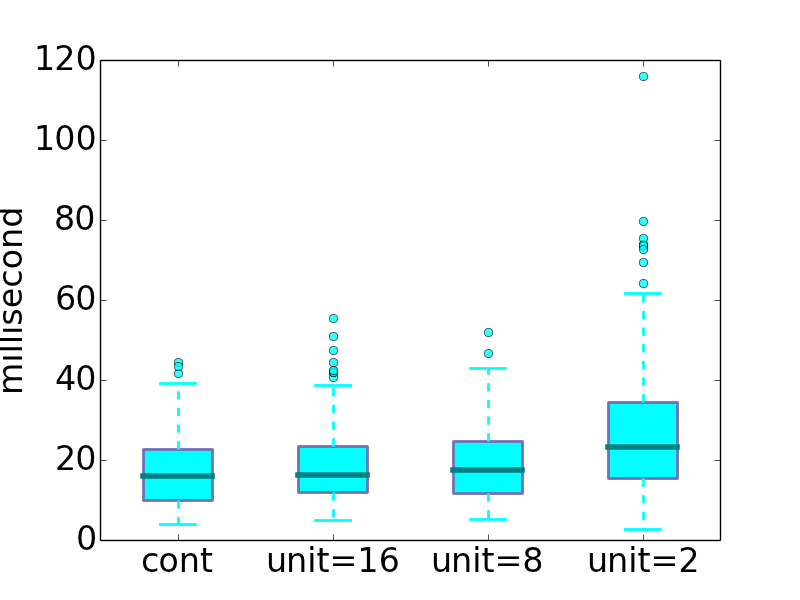
\includegraphics[height=1.5in]{figs/inter-job/amg}
        \caption{AMG}
        \label{fig:interjob-amg}
    \end{subfigure}%
    \hspace{1em}%
    \begin{subfigure}[t]{0.32\textwidth}
        \centering
        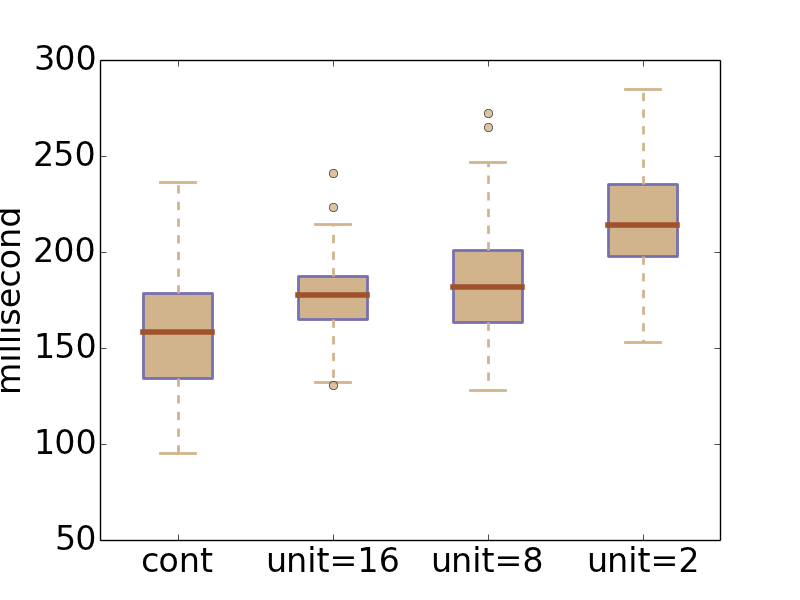
\includegraphics[height=1.5in]{figs/inter-job/cr}
        \caption{CrystalRouter}
        \label{fig:interjob-cr}
    \end{subfigure}%
    \begin{subfigure}[t]{0.32\textwidth}
        \centering
        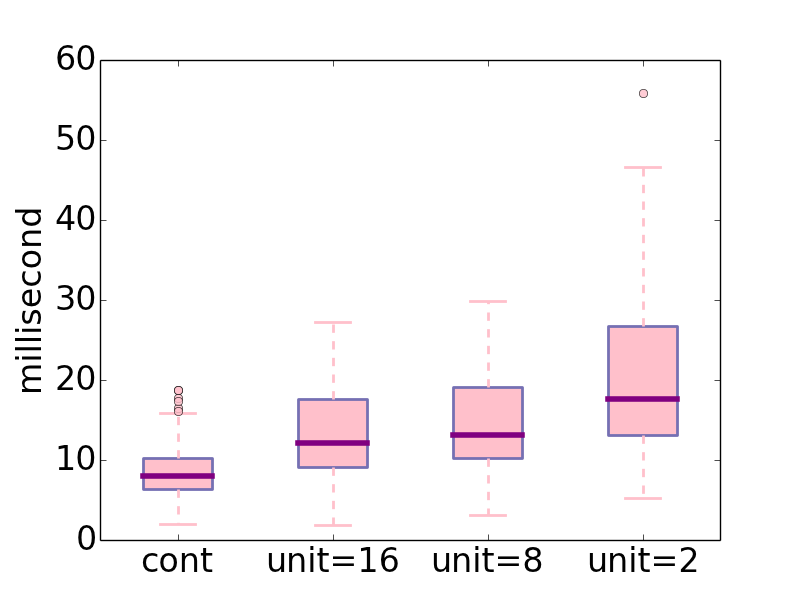
\includegraphics[height=1.5in]{figs/inter-job/mg}
        \caption{MultiGrid}
        \label{fig:interjob-mg}
    \end{subfigure}%
   \caption{
   Inter-job interference study. 
   ``cont" indicates three applications running side by side concurrently on the same network with contiguous allocation. 
   To study the impact of non-contiguous allocation on inter-job interference, 
   applications running concurrently with interleaved allocation of different unit sizes,
    which are 16-node, 8-node, 2-node. 
    }
   \label{fig:interjobstudy}
\end{figure*}

\subsection{Result Summary}
\label{sec:summary}

Based on the above comprehensive study, we can make following observations:

\begin{itemize}

    \item The compact allocation may not guarantee the best performance for every application. 
    
    \item The applications dominated with ``Nearest Neighbor" communications exhibit 
    relatively stable performance under different allocation shapes, 
    while the applications dominated with ``Many-to-Many" communication exhibit 
    better performance with compact allocation (e.g, 3D balanced).
    
    \item A good rank-to-node mapping strategy can greatly improve 
    application's performance when specific allocation is given.
    
    \item An optimal size for allocation units should be determined 
    according to an application's dominant communication pattern. 
    In general, a unit size should be large enough to accommodate  
    neighboring communication of the application. 
    
    \item Inter-job interference is inevitable in non-contiguous allocation. 
    However, choosing the proper allocation unit size with job's communication 
    pattern awareness can alleviate such negative effect. 
    
\end{itemize}







\section{Discussion}
\label{sec:discussion}

The results shown in the previous section provide insights for the design of smart and flexible job allocation. By scrutinizing job's communication behavior, we can identify job's dominant communication pattern and pinpoint the ``neighborhood communication". With such knowledge about jobs' communication patterns, we can analyze the possible interference between jobs and take precautions to alleviate the negative effect when making allocation decisions. 

When an application with dominant communication that is intensive ``Many-to-Many", the scheduler should grant it with compact node allocation and exclusive network provision. The compact allocation can guarantee the shortest pair-wise distance between all the ranks, and make the data transfer between ranks take less hops. On the other hand, the exclusive network provision will prevent other adjacent applications from sharing network resources, thus eliminate the performance degradation due to interference.

Not every application's preferable resource are compact node allocation and exclusive network provision. As we found in our analysis, applications whose dominant communication patterns contain intensive ``neighborhood communication" like ``Nearest Neighbor" don't benefit from compact node allocation and exclusive network provision. Applications, such as AMG, can run with non-contiguous node allocation without performance degradation, as long as the allocation unit can accommodate their ``neighborhood communication".

The allocation unit size shouldn't be fixed. Instead, the scheduler should choose a proper unit size based on the scale of ``neighborhood communication" of each job. The best unit size should be neither too big nor too small, jut perfectly fit for the size of that ``neighborhood". Big unit size won't be fully utilized and also cause fragmentation. Small unit size won't be able to accommodate the ``neighborhood communication" and makes the intra-job communication less efficient. 


The advantage of making allocation with consideration about job's communication pattern is obvious. First, compared with contiguous allocation policy, the new scheduler outlined above is more flexible, without requiring the system to provide a big contiguous partition to accommodate the whole application, it only needs to provide a small set of compact nodes that is sufficient for all the "local community" in the application. On the other hand, the new scheduler outlined above won't destroy the locality of application's communication pattern. Indeed, the small compact node set (allocation unit) provided for the application's  ``local communities" can preserve the communication locality in the maximum extent. The design of such a smart scheduler is part of our future work. 




\section{Related Work}
\label{sec:related_work}

There are many tools available for system monitoring and application profiling. 
Tools such as TAU (Tuning and Analysis)~\cite{tau} and mpiP~\cite{mpip} can capture 
application runtime information, keeping record in event traces. 
However, recognizing communication patterns from those traces require substantial effort. 
There are a number of studies on the recognition and characterization of parallel application communication patterns. 
Oak Ridge National Laboratory has an ongoing project about developing a tool set named Oxbow, 
which can characterize the computation and communication behavior of scientific applications and benchmarks~\cite{oxbow}. 
In a recent work~\cite{roth}, 
the authors demonstrate a new approach to automatically characterizing parallel applications communication behaviors. 

%\textbf{P2: communication characteristics}\\

Many research efforts have been conducted to characterize scientific applications. 
For instance, the DOE Design Forward Project aims to identify the 
computation and communication characteristics of a collection of relevant 
MiniApps developed at a number of exascale co-design centers~\cite{designforwardwebpage}. 
In this project, the communication patterns of several DOE full applications and associated 
mini-applications are studied to provide a more complete snapshot of DOE workloads. 
A joint project named CORAL from Oak Ridge, Argonne and Livermore provides a series of 
benchmarks to represent DOE workloads and technical requirements~\cite{coral}. 
The CORAL project includes scalable science benchmarks, throughput benchmarks, 
data centric benchmarks, skeleton benchmarks and micro benchmarks.  

%\textbf{P3: Interference between concurrently running jobs}\\
The interference among concurrently running jobs on HPC systems 
have been identified as major a culprit for job's performance variability. 
Bhatele et al. found that concurrently running applications interfere with each other, 
and cause their communication time varied from 
36\% shorter to 69\% longer on different HPC systems~\cite{abhinav-sc13}. 
Skinner et al. found that  there is a 2-3 times of slowdown in MPI$\textunderscore$Allreduce 
due to network contention from other concurrently running jobs~\cite{skinner}. 
%Rosenthal et al. found increasing network bandwidth provide limited benefits to a number of applications. 
%The applications that send mostly small messages or large messages asynchronously 
%are not bandwidth bounded, hence, benefit only slightly or not at all from increased bandwidth~\cite{rosenthal}.

%\textbf{P4: Job allocation(little bit)}\\
Several research studies focus on optimizing job allocation on HPC systems 
to alleviate the interference between concurrently running jobs. 
Hoefler et al. proposed to use performance modeling techniques to analyze factors that 
impact the performance of parallel scientific applications~\cite{hoefler-modeling}. 
However, as the scale of HPC systems continue to grow, 
the interference of concurrently running jobs is getting worse, 
which is hard to quantify with performance profiling tools alone. 
Bogdan et al. provide a set of guidelines on how to configure a Dragonfly network 
for workload with nearest neighbor communication pattern~\cite{Bogdan-hpdc14}. 
Dong et al. have developed simple benchmarks that conforms to four different communication patterns, 
namely ping-pong, nearest neighbor, broadcast and all$\textunderscore$reduce, 
to demonstrate the effectiveness of 5D torus networks~\cite{Dong-SC11}.

We differentiate our work from these works in the following ways. 
First, we focus on the dominant communication patterns rather than any specific application. 
We believe this can provide a guideline for other research work. 
Secondly, we explore \TODO{the} intra- and inter-job interference between concurrently running jobs, 
while similar work such as~\cite{abhinav-sc13} focuses 
on one single application's performance degradation due to network contention. 
Finally, we analyze the impact of different placement strategies to job's communication behaviors, 
identifying preferred placement strategies for 
each application with a specific dominant communication pattern. 
Based on our study, we claim that future batch schedulers should take 
job communication patterns into consideration for placement decision making. 


\section{Conclusions}
\label{sec:conclusion}
In this work, we have studied the communication behavior of three parallel applications, namely AMG, CrystalRouter and MultiGrid. Each application has distinctive communication pattern, that can be representative for a group of jobs in HPC workload. We have used a sophisticate simulation tool named CODES from Argonne National Laboratory to simulate the running of these three parallel applications on torus network. The torus network provided by CODES has good fidelity and scalability. We have analyzed the performance of each application's communication in terms of data transfer time by simulating them running on torus networks with different bandwidth and dimensionality configurations. We have found that higher dimensionality of torus network would improve the performance of application with ``Many-to-Many" communication patterns, while application with intensive local communication like ``Nearest Neighbor" won't benefit much from higher dimensionality.

We have analyzed the intra- and inter-job interference by simulating three applications running on 3D torus network. Based on our comprehensive experiments, we got five observations. 1) The compact allocation may not guarantee the best performance for every application. 2)The applications dominated with Nearest Neighbor communications exhibit relatively stable performance under different allocation shapes, while the applications dominated with Many-to-Many communication exhibit better performance with compact allocation (e.g. 3D balanced). 3) A good rank-to-node mapping strategy can greatly improve application's performance when specific allocation is given. 4) An optimal size for allocation units should be determined according to an application's dominant communication pattern. In general, a unit size should be large enough to preserve neighboring communication of the application. 5) Inter-job interference is inevitable in non-contiguous allocation. However, choosing the proper allocation unit size with job's communication pattern awareness can alleviate such negative effect.


We believe that our finding in this work can provide valuable guidance for HPC resource management to make flexible job allocations. Rather than using pre-defined partitions and non-contiguous allocation, future HPC systems should assign each job with preferable resources based on job's communication pattern. 




\section*{Acknowledgment}
\label{sec: ack}
The work at Illinois Institute of Technology is supported in part by U.S. National Science Foundation grants CNS-1320125 and CCF-1422009. This work is also supported by the U.S. Department of Energy, Office of Science, Advanced Scientific Computing Research, under Contract DE-AC02-06CH11357.

\bibliographystyle{IEEEtran}
\bibliography{IEEEabrv, reference}

\vspace{5\baselineskip}

\begin{framed}
The submitted manuscript has been created by UChicago Argonne, LLC, Operator of Argonne National Laboratory ("Argonne").  Argonne, a U.S. Department of Energy Office of Science laboratory, is operated under Contract No. DE-AC02-06CH11357.  The U.S. Government retains for itself, and others acting on its behalf, a paid-up nonexclusive, irrevocable worldwide license in said article to reproduce, prepare derivative works, distribute copies to the public, and perform publicly and display publicly, by or on behalf of the Government.
\end{framed}


\end{document}


